Our human beings can learn new things progressively in time. At a very young age, we can distinguish thousands of different objects and this ability can increasingly develop as we grow up. Moreover, we actually don't treat a new concept in isolation, but try to connect the new concept to the knowledge we already learned, which is referred to as transfer learning. For example, we recognize the animal zebra by referring it to the normal horse with distinctive black and white striped coats. Given a classification task of the target problem, transfer learning works on the scenario that knowledge learned from one or several prior (source) tasks can help the target learning task. 
Based on this, how to utilize the knowledge from multiple sources leads to the research of Multiple Source Transfer
Learning (MSTL). Transferring the knowledge from multiple priors can make the learning procedure extremely efficient by mining the recurrent patterns as well as inferring inductively on the target task \cite{tommasi2014learning}. Taking advantage of this, the first implementation proposed by \cite{fei2006one} using Bayesian approach shows that even with a single example, transfer learning can still get impressive results. Some methods using discriminative approach are proposed in recent years \cite{tommasi2014learning} \cite{kuzborskij2013n} \cite{jie2011multiclass}. Previous study shows that the more prior knowledge the system acquired, the easier a new concept can be learned \cite{Thrun96islearning}.

Transfer learning between different image databases is a very popular topic in recent years due to the fast growing vision-based applications. Multiclass incremental transfer learning (MITL) aims to add a new category model to the known source models by leveraging over them, while at the same time preserving their classification abilities \cite{kuzborskij2013n}. Based on this, we extend it to transfer the known source models to the identical target categories with different data distribution and add a new target category model as well. It is worthy to notice that when the data of the source and target tasks are drawn from the same distribution, our problem is decayed to the MITL problem. In MITL, it assumes that we can only access to the models of the source task rather than the original images. Following this setting, in our case, we have to face another challenge, negative transfer. Transferring knowledge can consistently boost the classification performance (positive transfer) is based on the fact that the learning procedure can benefit from sufficient related prior knowledge. In some situation, where the source domain and target one are not related, transferring the knowledge between them could even degrade the performance of the classifier of target task, which is referred to as negative transfer (see Figure \ref{fig:neg}). 
Negative transfer is a general issue even if we transfer knowledge between identical categories in different tasks due to the mismatched data distribution. In our case, the new added category could change the data distribution totally and transfer learning could more easily suffer from negative transfer (see Figure \ref{fig:distribution}). 
How to avoid negative transfer is still an open question in transfer learning \cite{Lu201514}. Specifically, how to the measure the transferability of different prior knowledge and obtain a comprehensive and accurate measurement to prevent negative transfer should be studied profoundly. Previous works suggest that, to better utilizing the prior knowledge to reduce negative transfer, decision of the algorithm should be made by combining the prior and empirical knowledge (knowledge obtained from specific target task) instead of aggressively ignoring or utilizing all the prior knowledge \cite{tommasi2014learning} \cite{kuzborskij2013n} \cite{yang2007cross} \cite{aytar2011tabula}.
\begin{figure}
\centering
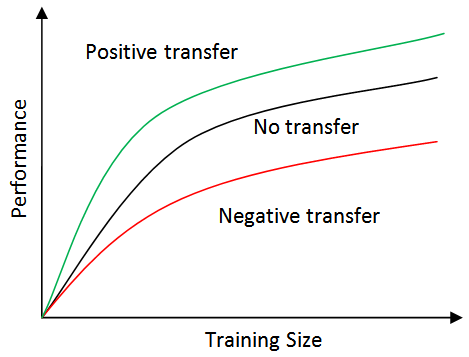
\includegraphics[scale=.5]{fig/negative.png}
\caption{Positive transfer VS Negative transfer. Relying on unrelated priors could lead to negative transfer.}\label{fig:neg}
\end{figure}
\begin{figure}
\centering
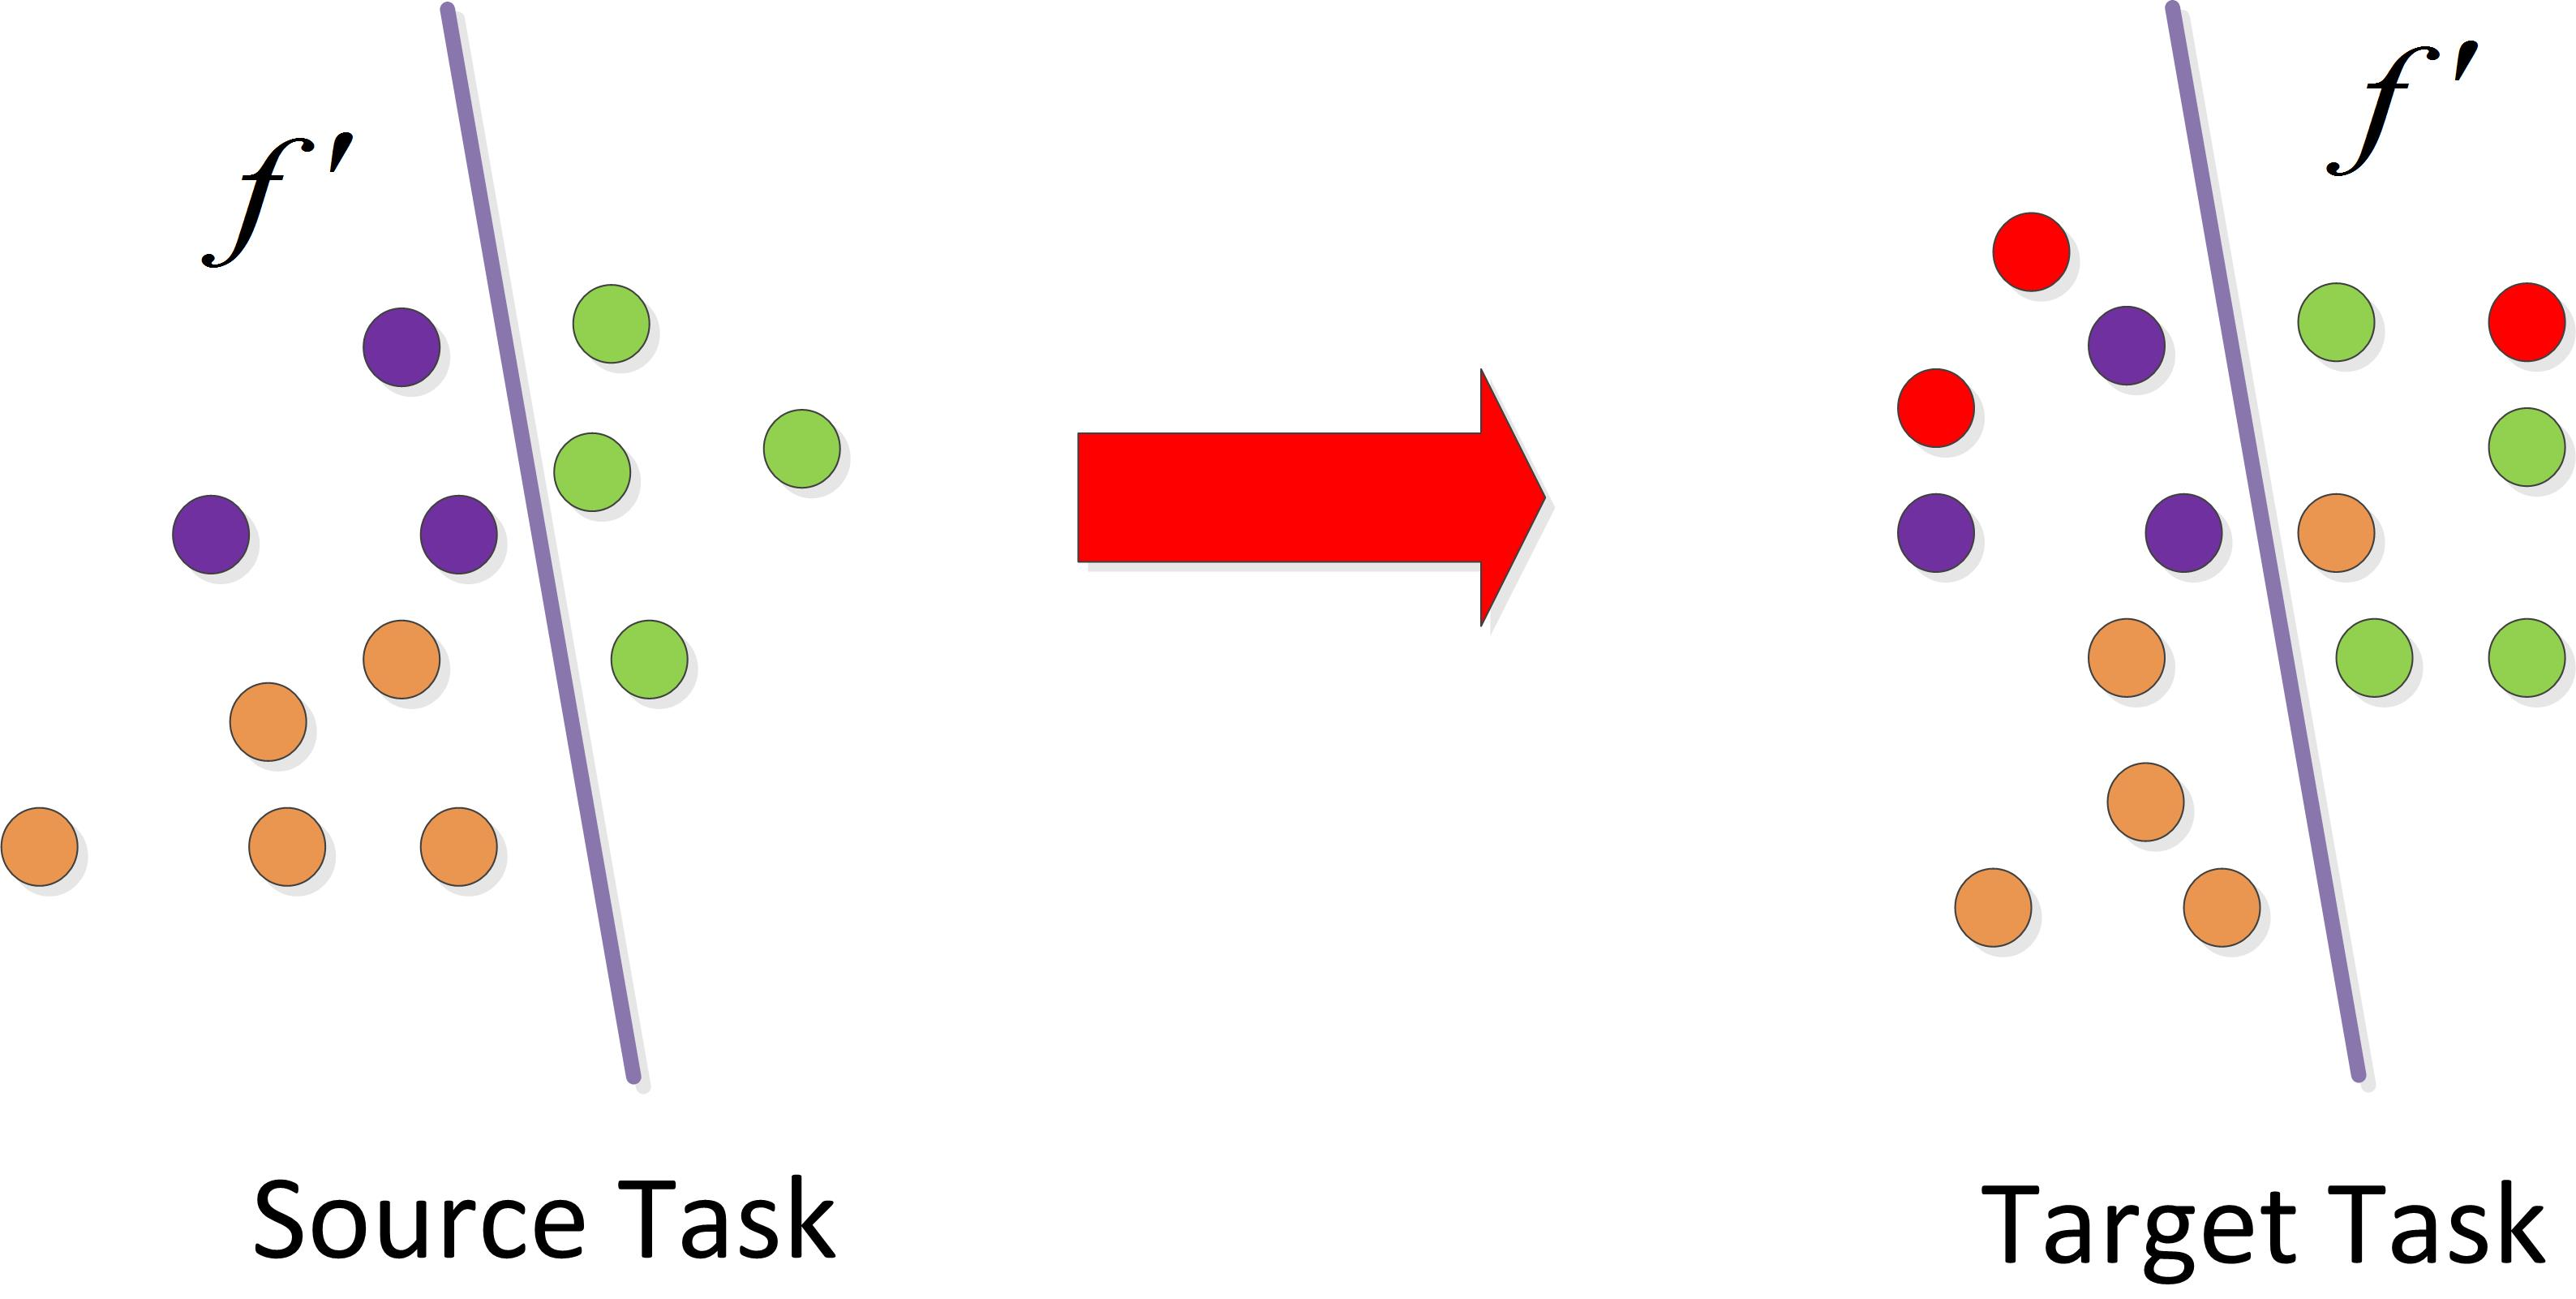
\includegraphics[scale=.4]{fig/domain.jpg}
\caption{Negative transfer may happen when we transfer prior knowledge $f'$ to target one. Points with different color represent different categories. The data distribution would change even for identical categories in different task. The red points denote the new category in target task. }\label{fig:distribution}
\end{figure}

In MITL, previous works focus on how to utilize the prior knowledge to preserve the performance for positive transfer rather than avoiding negative transfer. In our case, we focus on preventing negative transfer as well as boosting the performance for positive transfer. 
We use Least Square Support Vector Machine (LS-SVM) \cite{suykens1999least} as our basic model. The decision of each binary LS-SVM is the linear combination of the prior knowledge and empirical knowledge controlled by some transfer parameters. To measure the transferability of each prior knowledge, we estimate our transfer parameters using closed-form leave-one-out (LOO) error. Previous works theoretically suggest that closed-from LOO error can be an efficient way for parameter estimation with a small training set \cite{kuzborskij2013stability} \cite{cawley2006leave}. Then we propose our objective function that can balance the weight between the prior knowledge and empirical knowledge from target task. We also provide the theoretical proof that the transfer parameters optimized by our objective function can prevent negative transfer. Extensive empirical experiments show that other transfer learning baselines suffer from negative transfer while our method can autonomously ignore the unrelated prior knowledge to prevent negative transfer. Then, we also show that when the prior knowledge is highly related to the target task (positive transfer), our method can outperform the transfer learning baselines by aggressively utilizing the prior knowledge.

The rest of this paper is organized as follow:
  


%\begin{figure}
%\centering
%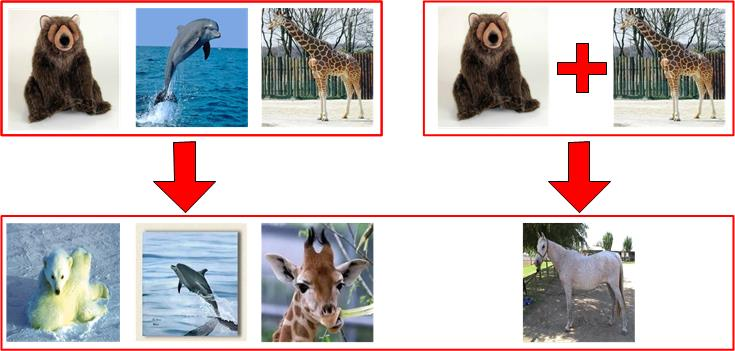
\includegraphics[scale=.4]{fig/transfer.jpg}
%\caption{}\label{fig:combine}
%\end{figure}